\pagestyle{fancy}
\setlength{\headheight}{16pt}
\fancyhead{} % clear all header fields
\fancyhead[L]{\textbf{CEE 576 Final II}}
\fancyhead[C]{Songyuan Cui}
\fancyhead[R]{\textbf{Fall 2024}}
\fancyfoot{} % clear all footer fields
\fancyfoot[C]{\thepage}

\section*{Errata regarding Part I}
The final results (Section 4) of Part I has maximum stresses and strains lowered by a factor of 10. 
The corrected figures up to maximum strain of $\sim 20\%$ are listed \href{https://github.com/sy-cui/CSE552-FA2024/tree/main/doc/final/part1}{here}.

\section{Dynamic formulation}
\subsection{Strong form}
Given the domain $\Omega$, desired time interval $(0, T)$, potentially time-dependent Dirichlet and Neumann boundaries $\Gamma_{g,i}$, $\Gamma_{j,i}$ and values $g_i$, $h_i$, external body forces $f_i$, and proper initial displacement and velocity $u_i^0$ and $v_i^0$, the strong form of the IBVP can be written as 
\begin{align}
    \rho \frac{\partial^2 u_i}{\partial t^2} &= \partial_j \sigma_{ij} + f_i, && \textrm{on} ~~ \Omega \times (0, T) \\
    u_i &= g_i(t), && \textrm{on} ~~ \Gamma_{g,i} \times (0, T) \\
    \sigma_{ij} n_j &= h_i(t), && \textrm{on} ~~ \Gamma_{h,i} \times (0, T) \\
    u_i(\bv{x}, 0) &= u_i^0(\bv{x}) && \textrm{on} ~~ \Omega_0 \\
    \frac{\partial u_i}{\partial t}(\bv{x}, 0) &= \dot{u}_i^0(\bv{x}) = v_i^0(\bv{x}) && \textrm{on} ~~ \Omega_0
\end{align}
where $\rho$ is the material density, and $\sigma_{ij}$ is the Cauchy stress tensor determined from $u_i$ (and $v_i$ for complex materials) via some constitutive relation. 

\subsection{Weak form}
Define the same trial and test spaces as previous assignments $\mathcal{S}$ and $\mathcal{V}$. 
The weak formulation is then as follows: find $u_i \in \mathcal{S}_i$ such that $\forall w_i \in \mathcal{V}_i$ satisfies
\begin{equation}\label{eqn:final2_weak_form_tdt}
    \int_{\Omega} w_i \rho \ddot{u}_i d\Omega + \int_{\Omega} w_{i,j} \sigma_{ij} d\Omega = \int_{\Omega} w_i f_i d\Omega + \sum_{i=1}^{N_{sd}} \int_{\Gamma_{h,i}} w_i h_i d\Gamma
\end{equation}
where $N_{sd}$ is the number of spatial dimensions.
Similar to Part I of the exam, this can alternatively be written in the reference or current configurations as 
\begin{subequations}
\begin{equation}\label{eqn:final2_weak_form_0}
    \int_{V} \rho_0 W_i \ddot{U}_i dV + \int_{V} W_{i,I} F_{iJ} S_{JI} dV = \int_{V} \rho_0 W_i B_i dV + \sum_{i=1}^{N_{sd}} \int_{A_{H,i}} W_i H_i dA,
\end{equation}
\begin{equation}\label{eqn:final2_weak_form_t}
    \int_{v} \rho_t w_i \ddot{u}_i dv + \int_{v} w_{i,j} \sigma_{i,j} dv = \int_{v} \rho_t w_i b_i dv + \sum_{i=1}^{N_{sd}} \int_{a_{h,i}} w_i h_i da.
\end{equation}
\end{subequations} 
where the definitions of variables are identical to those in Part I. 

\subsection{Time-continuous matrix form}
Without discretization in time, we write $u_i$ and $w_i$ within an element as linear combinations of basis functions $N_a(\bv{\xi})$:
\begin{equation}
    w_i^e (\bv{x}) = \sum_{a=1}^{N_{en}} c_{ia}^e N_a(\bv{\xi}), \quad u_i^e (\bv{x}) = \sum_{b=1}^{N_{en}} d_{ib}^e N_b(\bv{\xi})
\end{equation}
where $N_{en}$ is the number of nodes in each element. 
Substituting into \cref{eqn:final2_weak_form_0} or \cref{eqn:final2_weak_form_t} and assembling:
\begin{equation}\label{eqn:final2_eom}
\begin{gathered}
    \bt{M} \ddot{\bv{d}} + \bv{\Psi} (\bv{d}, \dot{\bv{d}}) = \bv{F}  \\
    \bt{M} = \assem_{e=1}^{N_{el}} \left[ \bt{M}^e \right], ~~~~ \bv{\Psi}(\bv{d}, \dot{\bv{d}}) = \assem_{e=1}^{N_{el}} \left[ \bv{\Psi}^e(\bv{d}^e, \dot{\bv{d}}^e) \right], ~~~~ \bv{F} = \assem_{e=1}^{N_{el}} \left[ \bv{F}^e \right]
\end{gathered}
\end{equation} 
where we have readily eliminated the test field nodal coefficients $c_{ia}$.
Here, $N_{el}$ is the total number of elements, and $\bt{\Psi}$ is the nonlinear internal force vector. 
Specifically, the element matrices / vectors can be written in integral forms: 
\begin{equation}\label{eqn:final2_element_matrices}
\begin{aligned}
    M_{iakb}^e &= \delta_{ik} \int_{V^e} \rho_0 N_a(\bv{\xi}(\bv{X})) N_b(\bv{\xi}(\bv{X})) dV \\
    \Psi_{ia}^e &= \int_{V^e} \frac{\partial N_a(\bv{\xi}(\bv{X}))}{\partial X_I} F_{iJ}(\bv{d}^e) S_{JI}(\bv{d}^e) dV  = \int_{v^e} \frac{\partial N_a(\bv{\xi} (\bv{x}))}{\partial x_j} \sigma_{ij}(\bv{d}^e) dv \\
    F_{ia}^e &= \int_{V^e} \rho_0 N_a(\bv{\xi}(\bv{X})) B_i dV + \int_{A_{H,i}^e} N_a(\bv{\xi}(\bv{X})) H_i^e dA \\
    &= \int_{v^e} \rho_t N_a(\bv{\xi}(\bv{x})) b_i dV + \int_{a_{h,i}^e} N_a(\bv{\xi}(\bv{x})) h_i^e da \\
\end{aligned}
\end{equation}
Note that the indices combination such as $ia$ can be consolidated into one via a numbering system such as 
\begin{equation}
p = N_{sd} (a - 1) + i, ~~~~ q = N_{sd} (b - 1) + k
\end{equation}
such that fourth-order tensors (e.g. $M_{iakb}^e$) become rank-2 matrices, and matrices (e.g. $F_{ia}^e$) become vectors.

The consistent tangent, obtained by taking the variational derivative of $\bt{\Psi}$ with respect to the displacement field, is identical to that derived in Part I.
In the current configuration, the variational derivative is written as 
\begin{equation}
    D\psi(\bv{x}) \cdot \bv{\Delta \bv{u}} = \int_v w_{i,j} \Delta u_{k,l} \left( c_{ijkl} + \delta_{ik} \sigma_{jl} \right) dv,
\end{equation}
and the consistent tangent matrix is 
\begin{equation}
    K_{iakb} = \int_v \frac{\partial N_a}{\partial x_j} \left( c_{ijkl} + \delta_{ik} \sigma_{jl} \right) \frac{\partial N_b}{\partial x_l} dv.
\end{equation}
where $c_{ijkl}$ and $\sigma_{jl}$ should be evaluated from the currently known displacement (and, if necessary, velocity) field via constitutive relations. 
\emph{These relations are all listed in Part I and thus not repeated here}. 

\section{Mass matrix}
We henceforth assume $\rho_0 = 1$. 
The mass matrix, due to mass conservation, must remain constant in time.
Hence, it is sufficient to compute it \emph{once} in the reference configuration which is readily shown in \cref{eqn:final2_element_matrices}. 
Specifically, it derives from the weak form as 
\begin{equation}
\begin{aligned}
    \int_{V^e}  \rho_0 W_i \ddot{U}_i dV 
    &= \int_{V^e} \left( \sum_{a=1}^{N_{en}} c_{ia}^e N_a(\bv{\xi})\right)\left(\sum_{b=1}^{N_{en}} d_{ib}^e N_b(\bv{\xi}) \right) dV \\
    &= \sum_{a=1}^{N_{en}} \sum_{b=1}^{N_{en}} c_{ia}^e \underbrace{\left[ \delta_{ik} \int_{V^e} N_a(\bv{\xi})N_b(\bv{\xi}) dV \right]}_{M_{iakb}^e} d_{kb}^e \\
\end{aligned}
\end{equation}
Given a square element of size $1 \times 1$, the mass matrix can be easily computed by hand. 
First, due to the presence of $\delta_{ik}$, $\bt{M}^e$ can be written in tensor product form $\bt{m}^e \otimes \bt{I}_2$, where 
\begin{equation}
\begin{aligned}
    m_{ab}^e &= \frac{dX}{dr} \frac{dY}{ds} \int_{-1}^1 \int_{-1}^1 N_a(r, s) N_b(r, s) dr ds  \\
    & = \frac{1}{4} \int_{-1}^1 \int_{-1}^1 N_a(r, s) N_b(r, s) dr ds \\
\end{aligned}
\end{equation}
and 
\begin{equation}
    N_1(r,s) = \frac{(1-r)(1-s)}{4}, ~~ N_2(r,s) = \frac{(1+r)(1-s)}{4}, ~~ N_3(r,s) = \frac{(1+r)(1+s)}{4}, ~~ N_4(r,s) = \frac{(1-r)(1+s)}{4}
\end{equation}
The resulting element mass matrix is then 
\begin{equation}
    \bt{M}^e = \bt{m}^e \otimes \bt{I}_2 = \frac{1}{36}\begin{bmatrix}
        4 & 0 & 2 & 0 & 1 & 0 & 2 & 0 \\
          & 4 & 0 & 2 & 0 & 1 & 0 & 2 \\
          &   & 4 & 0 & 2 & 0 & 1 & 0 \\
          &   &   & 4 & 0 & 2 & 0 & 1 \\
          &   &   &   & 4 & 0 & 2 & 0 \\
          &   &  \multirow{2}{*}{\makebox[0pt]{\text{sym.}}} &   &   & 4 & 0 & 2 \\
          &   &   &   &   &   & 4 & 0 \\
          &   &   &   &   &   &   & 4 \\
    \end{bmatrix}
\end{equation}
The row-sum lumped mass matrix is then simply $\bt{M}_l^e = \textrm{diag}\{0.25\} \in \mathbb{R}^{8\times 8}$. 

\section{Time integration}
The HHT-$\alpha$ method for the nonlinear dynamic problem \cref{eqn:final2_eom} is 
\begin{gather}
    \label{eqn:final2_hht} \bt{M} \bv{a}_{n+1} + (1+\alpha) \bv{\Psi}(\bv{d}_{n+1}, \bv{v}_{n+1}) = \bt{F}_{n+\alpha} + \alpha \bt{\Psi}(\bv{d}_n, \bv{v}_n) \\
    \bv{d}_{n+1} = \bv{d}_n + \Delta t \bv{v}_n + \frac{\Delta t^2}{2} \left[ (1-2\beta) \bv{a}_n + 2\beta \bv{a}_{n+1} \right] \\
    \bv{v}_{n+1} = \bv{v}_n + \Delta t \left[ (1-\gamma) \bv{a}_n + \gamma \bv{a}_{n+1} \right]
\end{gather}
for which stability is ensured if $\alpha \in [-1/3, 0]$, $\beta={(1-\alpha)}^2/4$, and $\gamma = (1-2\alpha) / 2$.
In the context of predictor-(multi)corrector methods, we define the predictors 
\begin{equation}
\begin{aligned}
    \tilde{\bv{d}}_{n+1} &= \bv{d}_n + \Delta t \bv{v}_n + \frac{\Delta t^2}{2} (1 - 2\beta) \bv{a}_n \\
    \tilde{\bv{v}}_{n+1} &= \bv{v}_n + \Delta t (1 - \gamma) \bv{a}_n
\end{aligned}
\end{equation}
and correctors 
\begin{equation}
\begin{aligned}
    \bv{d}_{n+1} &= \tilde{\bv{d}}_{n+1} + \beta \Delta t^2 \bv{a}_{n+1}\\ 
    \bv{v}_{n+1} &= \tilde{\bv{v}}_{n+1} + \gamma \Delta t \bv{a}_{n+1}
\end{aligned}
\end{equation}
Next, we linearize the nonlinear internal force vector $\bv{\Psi}$ about the predictor values:
\begin{equation}
\begin{aligned}
    \bv{\Psi}(\bv{d}_{n+1}, \bv{v}_{n+1}) &= \bt{\Psi}(\tilde{\bv{d}}_{n+1}, \tilde{\bv{v}}_{n+1}) + \frac{\partial \bv{\Psi}}{\partial \bv{d}} \Big|_{\bv{d}=\tilde{\bv{d}}_{n+1}} (\bv{d}_{n+1} - \tilde{\bv{d}}_{n+1}) + \frac{\partial \bv{\Psi}}{\partial \bv{v}} \Big|_{\bv{v}=\tilde{\bv{v}}_{n+1}} (\bv{v}_{n+1} - \tilde{\bv{v}}_{n+1}) + h.o.t. \\
    &= \bt{\Psi}(\tilde{\bv{d}}_{n+1}, \tilde{\bv{v}}_{n+1}) + \beta \Delta t^2 \bt{K}_n \bv{a}_{n+1} + \gamma \Delta t \bt{C}_n \bv{a}_{n+1} + h.o.t. \\
\end{aligned}
\end{equation}
Substituting back into \cref{eqn:final2_hht} and rearranging yields the update formula:
\begin{equation}
\begin{gathered}
    \bt{M}^* \bv{a}_{n+1} = \bv{R}_{n+\alpha} \\
    \bv{R}_{n+\alpha} = \left[(1+\alpha)\bv{F}_{n+1} - \alpha\bv{F}_n\right] - \left[(1+\alpha)\bv{\Psi}(\tilde{\bv{d}}_{n+1}, \tilde{\bv{v}}_{n+1}) - \alpha\bv{\Psi}(\bv{d}_n, \bv{v}_n) \right] \\
    \bt{M}^* = \bt{M} + (1+\alpha)(\beta \Delta t^2 \bt{K}_n + \gamma \Delta t \bt{C}_n)
\end{gathered}
\end{equation}
where we may treat $\bv{a}_{n+1}$ as an known to solve for iteratively.
The multi-corrector strategy is to the embed (modified) Newton-Raphson iteration into the above algorithm, where we successively update the predictors $\tilde{\bv{d}}_{n+1}$ and $\tilde{\bv{v}}_{n+1}$ (and thus the residual) to solve for the corrector $\Delta \bv{a}_{n+1}$.

\emph{Instead of a flow chart, the detailed procedure is formulated in pseudocode format} in \cref{alg:final2_pmc}. 
Note that the modified Newton-Raphson method is employed. 
To adjust the algorithm for the Newton-Raphson method, one needs simply recompute the tangent $\bt{K}$ and damping $\bt{C}$ matrices after each iteration (\code{while}-loop).  

\begin{algorithm}[!ht]
\caption{One time-step of the predictor-multicorrector $\alpha$-method for nonlinear dynamics}
\begin{algorithmic}\label{alg:final2_pmc}
    \setlength{\lineskip}{8pt}

    \Require{Nonlinear function $\bt{\Psi}(\bv{d}_n, \bv{v}_n)$, last known kinematic values $\bv{u}_n$, $\bv{v}_n$, $\bv{a}_n$, external forces $\bv{F}_n$ and $\bv{F}_{n+1}$, mass matrix $\bt{M}$, consistent tangent $\bt{K}_n$, damping matrix $\bt{C}_n$, time step $\Delta t$, $\alpha$, $\beta$, $\gamma$, tolerance $\epsilon$}

    \Ensure{Approximated solution at time $t + \Delta t$}
    
    \State{$\bt{M}^* \gets \bt{M} + (1+\alpha) \left( \beta \Delta t^2 \bt{K}_n + \gamma \Delta t \bt{C}_n \right)$}
    \Comment{Effective mass matrix}

    \State{$\bv{d}_{n+1}^{(0)} \gets \bv{d}_n + \Delta t \bv{v}_n + \frac{\Delta t^2}{2} (1 - 2\beta) \bv{a}_n$}
    \Comment{Displacement predictor}

    \State{$\bv{v}_{n+1}^{(0)} \gets \bv{v}_n + \Delta t (1 - \gamma) \bv{a}_n$}
    \Comment{Velocity predictor}

    \State{$\bv{a}_{n+1}^{(0)} \gets \bv{0}$}

    \State{$\bv{R}_{n+\alpha}^{(0)} \gets \left[(1+\alpha)\bv{F}_{n+1} - \alpha\bv{F}_n \right] - \left[(1+\alpha)\bv{\Psi}(\bv{d}_{n+1}^{(0)}, \bv{v}_{n+1}^{(0)}) - \alpha\bv{\Psi}(\bv{d}_n, \bv{v}_n) \right]$}
    \Comment{Initial residual}

    \State{$i \gets 0$}

    \While{$\| \bv{R}_{n+\alpha}^{(i)} \| / \| \bv{R}_{n+\alpha}^{(0)} \| > \epsilon $}

    \State{Solve $\bt{M}^* \Delta \bv{a}_{n+1}^{(i)} = \bv{R}_{n+\alpha}^{(i)}$}

    \State{$\bv{a}_{n+1}^{(i+1)} \gets \bv{a}_{n+1}^{(i)} + \Delta \bv{a}_{n+1}^{(i)}$}

    \State{$\bv{d}_{n+1}^{(i+1)} \gets \bv{d}_{n+1}^{(i)} + \beta \Delta t^2 \Delta \bv{a}_{n+1}^{(i)}$}
    \Comment{Displacement corrector}

    \State{$\bv{v}_{n+1}^{(i+1)} \gets \bv{v}_{n+1}^{(i)} + \gamma \Delta t \Delta \bv{a}_{n+1}^{(i)}$}
    \Comment{Velocity corrector}

    \State{$\bv{R}_{n+\alpha}^{(i+1)} \gets \left[(1+\alpha)\bv{F}_{n+1} - \alpha\bv{F}_n \right] - \left[(1+\alpha)\bv{\Psi}(\bv{d}_{n+1}^{(i+1)}, \bv{v}_{n+1}^{(i+1)}) - \alpha\bv{\Psi}(\bv{d}_n, \bv{v}_n) \right] - \bt{M} \bv{a}_{n+1}^{(i+1)}$}

    \State{$i \gets i + 1$}

    \EndWhile{}

    \State{$\bv{d}_{n+1} \gets \bv{d}_{n+1}^{(i)}$,~~~~$\bv{v}_{n+1} \gets \bv{v}_{n+1}^{(i)}$,~~~~$\bv{a}_{n+1} \gets \bv{a}_{n+1}^{(i)}$}

\end{algorithmic}
\end{algorithm}

\section{Numerical results}

In this section, we examine the dynamical solution of the two given scenarios with the HHT-$\alpha$ method at $\alpha=0$ and $\alpha = -1/3$, respectively. 
The material property for both cases is set to $E = \qty{10}{\pascal}$, $\nu = 0.25$, $\rho = \qty{1}{\kg\per\m\cubed}$, and $t = \qty{1}{\m}$.
\emph{Note that the Young's modulus has been reduced by a factor of $10^7$ compared with Part I for two reasons: }
\begin{itemize}
    \item {
        High stiffness leads to high natural frequency of the material ($\omega \sim \sqrt{E / \rho L^2}$), which requires \emph{very small time steps} to resolve correctly and avoid aliasing. 
        Moreover, the result is not graphically meaningful due to the shear number of periods within the simulation time interval.
    }
    \item {
        Possibly due to the nonlinearity of the problem, the high stiffness appears to lead to numerical instability despite the unconditionally stable time-stepping scheme.
    }
\end{itemize}
It is also worth noting that the obtained solution for the single element is not faithful to the actual response of the modeled material even in the linear elastic case (e.g. the configuration shown in (b) does not match the expected solution to the corresponding wave equation, but it is rectified after increasing the number of elements). 

All implementations can be found at \href{https://github.com/sy-cui/CSE552-FA2024/tree/main/final/part2}{the linked repository}.
Please refer to the \code{README.md} file in the same directory for code instructions. 

\subsection{Scenario (b): stretch}

We first ``stretch'' the material such that the $Y$ position of node 3 and 4 are at $Y = 1.2$, and thus the $X$ position of these two nodes will not remain at $0$ and $1$. 
We then release this ``stretching'' boundary condition and time-integrate the system to $t = 10$ using a uniform time step of $\Delta t = 10^{-3}$.
The displacement and velocity of node 3 (north west node) is shown in \cref{fig:final2_stretch_0,fig:final2_stretch_3} for $\alpha = 0$ and $\alpha = -1/3$, respectively.

We remark the the energy of the system appears to be conserved, as expected from the trapezoidal rule. 
However, using $\alpha = -1/3$ \emph{does not appear to introduce any numerical dissipation}. 
This is likely due to the fact that the damping effect of the HHT method applies primarily to high-frequency modes (typically above a critical frequency that is $\alpha$-dependent). 
The system does not have a dominant highly-oscillatory mode for the $\alpha$-method to attack, and thus the damping effect is not pronounced.

\begin{figure}[!ht]
    \centering
    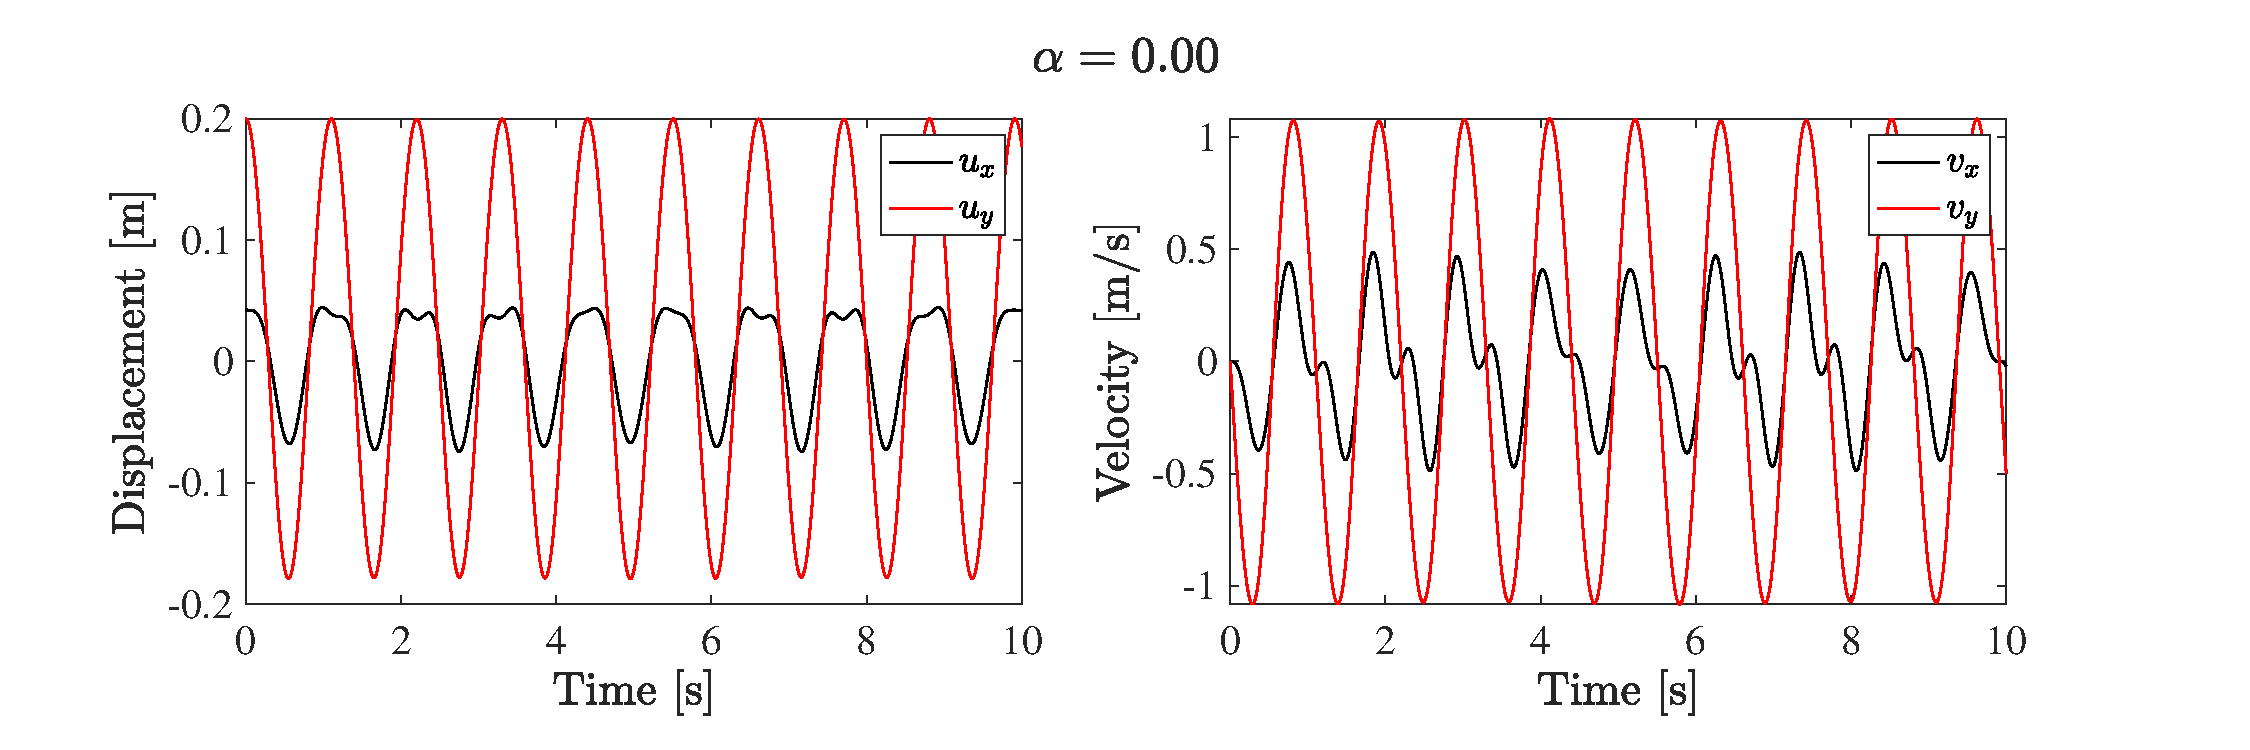
\includegraphics[width=\textwidth]{final/part2/final2_stretch_0.pdf}
    \caption{Displacement and velocity of node 3 for part (b) at $\alpha = 0$.}
    \label{fig:final2_stretch_0}
\end{figure}

\begin{figure}[!ht]
    \centering
    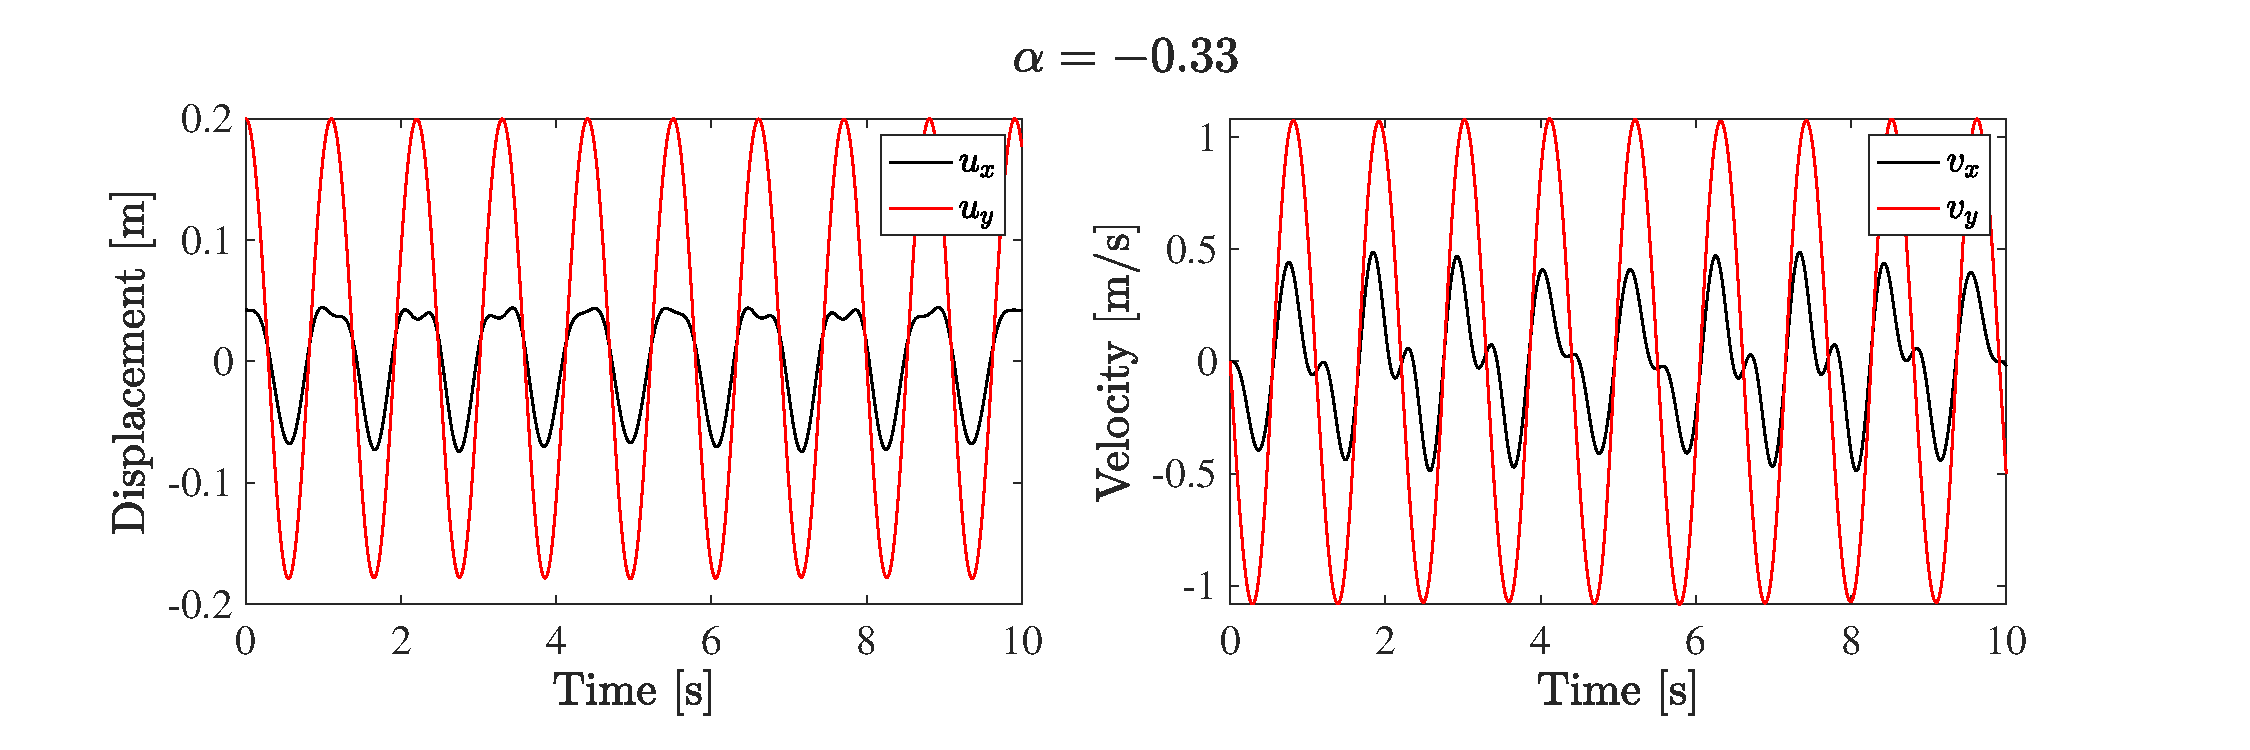
\includegraphics[width=\textwidth]{final/part2/final2_stretch_333.pdf}
    \caption{Displacement and velocity of node 3 for part (b) at $\alpha = -1/3$.}
    \label{fig:final2_stretch_3}
\end{figure}

\subsection{Scenario (c): shear}
Here we apply a shear deformation to the material by displacing the $X$ position of node 3 and 4 by $0.2$, without imposing any condition upon the $Y$ position. 
Similarly, the boundary condition is then released and time-marched to $t = 10$ with a uniform time step of $\Delta t = 10^{-3}$.
The three Cauchy-stress components at the third quadrature node in the provided figure (4th node in the code) are shown in \cref{fig:final2_shear_0,fig:final2_shear_3} for $\alpha = 0$ and $\alpha = -1/3$, respectively.

Again, we see no significant difference in the results between the two $\alpha$ values likely for the same reason as in the previous scenario. 
Aligned with the observations from Part I, $\sigma_{22}$ is the most prominent stress component, and hence with the highest oscillatory amplitude. 
THe other two components are similar in magnitude and oscillating in phase with $\sigma_{22}$.

\begin{figure}[!ht]
    \centering
    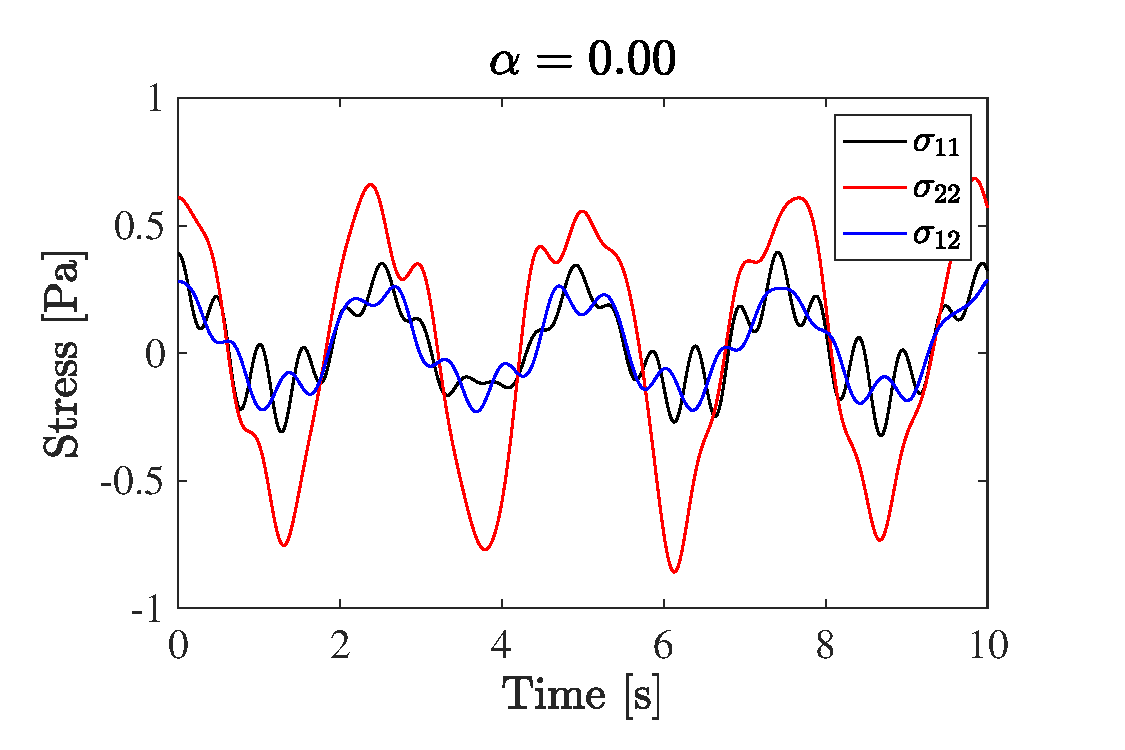
\includegraphics[width=0.6\textwidth]{final/part2/final2_shear_0.pdf}
    \caption{Cauchy stress components at node 3 for part (c) at $\alpha = 0$.}
    \label{fig:final2_shear_0}
\end{figure}

\begin{figure}[!ht]
    \centering
    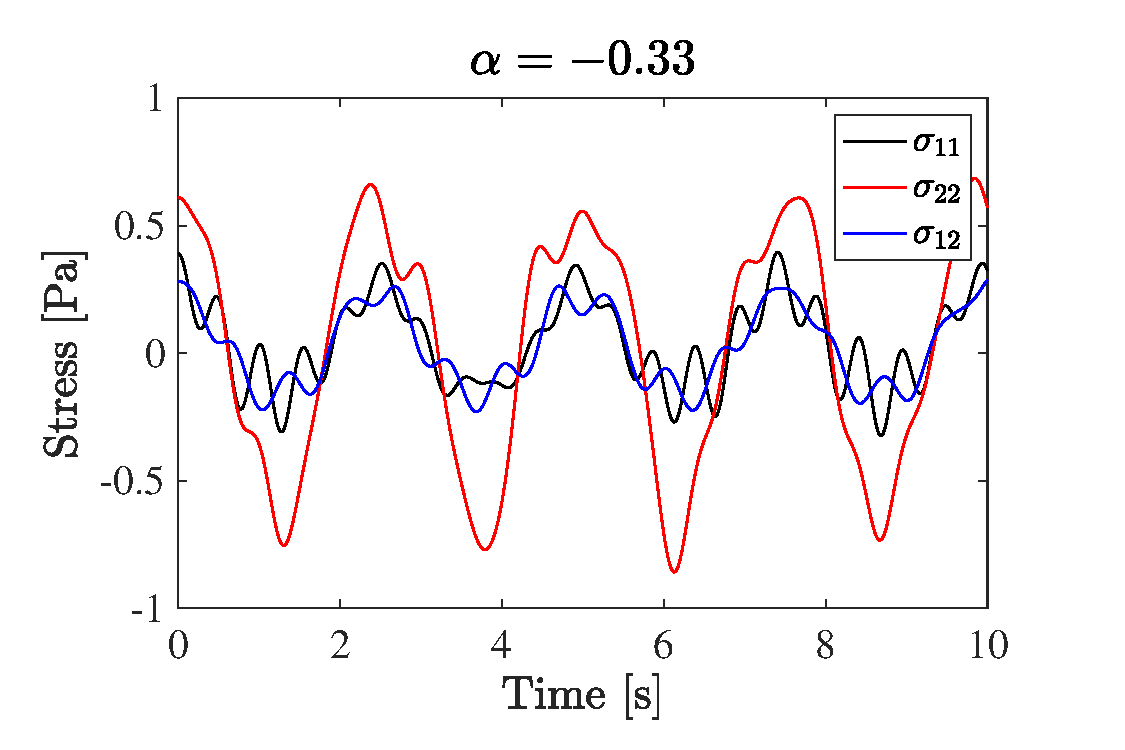
\includegraphics[width=0.6\textwidth]{final/part2/final2_shear_333.pdf}
    \caption{Cauchy stress components at node 3 for part (c) at $\alpha = -1/3$.}
    \label{fig:final2_shear_3}
\end{figure}